\chapter{Evaluation}

In this chapter, we will evaluate Psnodig against the goals we set in Section 1. The goals focused on Psnodig being extensible, executable, and presentable. \\

Psnodig is extensible if we are able to add parsers and code generators (also referred to as \textit{writers}) to it. Psnodig is executable if we are able to run their source code. This means that, technically, Psnodig cannot be executable if it is not also extensible. Lastly, Psnodig is presentable if we are able to convert the original source code to different levels of abstraction, more specifically pseudocode and flowcharts. \\

To keep a common thread going through this chapter, we will use selected algorithms from Algorithm Design and Applications by
Michael T. Goodrich and Roberto Tamassia as a case study~\cite{pseudocodeInBook2}. The algorithms will span across a diverse section of algorithm categories, presented in greater detail below.

\subsubsection{Search Algorithms}

Sorting algorithms aim to find a particular element in a list, and we have selected two for evaluation: naive search and binary search. Despite having the same goal, they differ sligthly in complexion. \\

Naive search iteratest the list sequentially. It works on all lists, since in the worst case it will check every element. Binary search starts in the middle and excludes half the list in each iteration. As such, it relies on the list being ordered.

\subsubsection{Binary Search Trees Algorithms}

Binary search trees (BST) are a common data structure in computer science. Each node has at most two child nodes, and all nodes are descendents of a single root node. Additionally, for all nodes \textbf{nd}, every node to the left of \textbf{nd} must have a value smaller than or equal to \textbf{nd}, and every node to the right must have a value greater than or equal to \textbf{nd}. \\

We have selected four algorithms related to BST for evaluation: find max, insert, remove, and search. \\

Find max will find the largest value in a given BST, starting from the root node. Insert will insert a node in its correct place in a given BST, according to its value. Remove will remove a node from a given BST, whilst preserving the tree's properties. Lastly, search will search through the tree for a node with a particular value, and return it if it exists.

\subsubsection{Sorting Algorithms}

Sorting algorithms take a list as input, and return the list with elements sequenced from smallest to greatest. We have selected three for evaluation: bubble sort, quicksort, and bucket sort. \\

Bubble sort compares the elements on index 0 and 1, and if the first is larger than the second, they are swapped. It continues to compare the elements on index 1 and 2, and so on. This iteration occurs n times, where n equals the length of the list minus one. In each passing, the unsorted largest element in the list is placed in its proper position towards the end of the list. \\

Quicksort is a recursive algorithm. It chooses a pivot element, before placing all smaller elements on its left and all larger elements on its right (without sorting them). Then it does this recursively for the lists on each side of the pivot, until we have looked at every integer in the list. Lastly, it merges these sub-lists together, resulting in an ordered list. \\

Bucket sort has an entirely different approach. It creates N empty lists, corresponding to a certain key. Then, all elements are put in the list they belong to, and the lists are sorted individually. Lastly, it iterates each list from number 0 to number N sequentially, adding the elements back to the list in an ordered fashion.

\subsubsection{Graph Algorithms}

Graphs are made up of two parts: nodes and edges. Nodes represent objects, and edges are the links between them. They are useful due to the large amount of data that can be represented as a graph, as well as the existing algorithms that are able to efficiently process that data. \\

However, many graph algorithms rely on implementations of a priority queue, that we did not have time to implement. Therefore, we selected two algorithms for evaluation: breadth-first search, and depth-first search. \\

Breadth-first search (BFS) and depth-first search (DFS) are algorithms for traversing graphs, and are commonly used to identify all nodes within a connected component. They only differ in the internal data structure they use: BFS uses a queue, whilst DFS uses a stack. \\

Since Psnodig does not currently support queue operations like removing the first element in a list, we implemented one ourselves for the sake of evaluating BFS.

\section{Extensible}

The first goal of Psnodig is extensibility: we should be able to add parsers and writers to Psnodig. The parsers must take a source program and convert it to an internal representation. The writers must take an internal representation and convert it to a program. \\

We have written a parser for an imperative, C-like programming language that we coined \textbf{Gourmet}. We have also written two writers: one that produces Gourmet programs, and one that produces Python programs.

\subsection{Gourmet Parser}

What we aim to evaluate here, is whether or not the parser is compatible with Psnodig. The Psnodig grammar is a limitation of how rich a program can look before it is converted by a writer. This means that a parser can at most parse all data types, but at the very least a \texttt{Program}, as it is the entry point of all Psnodig programs. \\

A minimal example is an empty program. The Gourmet parser is capable of parsing empty files, producing an AST of a \texttt{Program Nothing [] [] Nothing} value. We cannot produce a maximal example, because \texttt{Program} contains a list of \texttt{FunctionDecl} values, that again contain a list of \texttt{Statement} values. These values can be compound, and in effect go on forever.\footnote{We could interpret a maximal example to be a program limited by our computer’s memory, but theoretically Psnodig programs can be infinitely big.} \\

To evaluate if we have successfully extended Psnodig with a parser, we will implement the four algorithms. We will then run them on a function that parses the programs, and produces either a Psnodig AST or a parse error. \\

As programs increase in size and complexity, so do Psnodig ASTs. For the sake of readability, we will only present the one in \Cref{naiveSearchAST} here. This is also because the ASTs will have a similar structure, and we believe that one is sufficient to represent them. The remaining ASTs can be found in \Cref{appendixA}.

\subsubsection{Search Algorithms}

\begin{lstlisting}[caption={Naive search implementation in Gourmet.}, captionpos=b, label={naiveSearchGourmet}]
? A list A and an integer x?
! True if x $\$$\in$\$$ A and false if not!

func NaiveSearch(A list, x int) {
    for i := A {
        if i == x {
            return true
        }
    }
    return false
}
\end{lstlisting}

\begin{lstlisting}[caption={The Psnodig AST generated by parsing \Cref{naiveSearchGourmet}.}, captionpos=b, label={naiveSearchAST}]
Program
  (Just (ProgramDescription
    "A list A and an integer x"
    "True if x $\$$\in$\$$ A and false if not"))
  []
  [ FunctionDecl
      "NaiveSearch"
      [ Argument "A" "list", Argument "x" "int" ]
      [ ForEach
          "i"
          (VariableExp "A")
          [ If
              (BinaryExp Equal
                (VariableExp "i")
                (VariableExp "x"))
              [Return (Constant (Boolean True))]
              Nothing
          ],
        Return (Constant (Boolean False))
      ]
  ]
  Nothing
\end{lstlisting}

\begin{lstlisting}[caption={Binary search implementation in Gourmet.}, captionpos=b, label={binarySearchGourmet}]
? A list A and an integer x?
! True if x $\in$ A and false if not!

func BinarySearch(A list, x int) {
    low := 0
    high := length(A) - 1

    while low <= high {
        i := floor((low + high) / 2)

        if A[i] == x {
            return true
        }
        else if A[i] > x {
            high := i - 1
        }
        else {
            low := i + 1
        }
    }
    return false
}
\end{lstlisting}

\newpage

\subsubsection{Binary Search Tree Algorithms}

\begin{lstlisting}[caption={Find max in BST implementation in Gourmet.}, captionpos=b, label={findMaxGourmet}]
? A binary search tree $t$?
! The node with the largest value in $t$!

struct Tree {
    value int,
    left Tree,
    right Tree
}

func FindMax(t Tree) {
    if t == nil {
        return nil
    }

    if (t.right) == nil {
        return t
    }

    return FindMax(t.right)
}
\end{lstlisting}

\begin{lstlisting}[caption={Insert in BST implementation in Gourmet.}, captionpos=b, label={insertGourmet}]
? A binary search tree $t$ and an integer $val$?
! $t$ with a node of value $val$!

struct Tree {
    value int,
    left Tree,
    right Tree
}

func Insert(t Tree, val int) {
    if t == nil {
        t := struct Tree(val, nil, nil)
    }
    else if val < (t.value) {
        t.left := Insert(t.left, val)
    }
    else if val > (t.value) {
        t.right := Insert(t.right, val)
    }

    return t
}
\end{lstlisting}

\begin{lstlisting}[caption={Deletion in BST implementation in Gourmet.}, captionpos=b, label={removeGourmet}]
? The root node in a tree and the value of a node to be deleted?
! The updated tree with one less node!

struct Tree {
    value int,
    left Tree,
    right Tree
}

func Delete(node Tree, val int) {
    if node == nil {
        return nil
    }
    else if (node.value) < val {
        node.right := Delete(node.right, val)
        return node
    }
    else if (node.value) > val {
        node.left := Delete(node.left, val)
        return node
    }

    if (node.left) == nil {
        return node.right
    }
    else if (node.right) == nil {
        return node.left
    }

    node' := FindMax(node.left)
    node.value := node'.value
    node.left := Delete(node.left, node.value)
    return node
}

func FindMax(root Tree) {
    if (root.right) == nil {
        return (root.value)
    }

    return FindMax(root.right)
}
\end{lstlisting}

\begin{lstlisting}[caption={Search in BST implementation in Gourmet.}, captionpos=b, label={searchGourmet}]
? A binary search tree $t$ and an integer $val$?
! True if $val \in t$ and False if not!

struct Tree {
    value int,
    left Tree,
    right Tree
}

func Search(t Tree, val int) {
    if t == nil {
        return false
    }
    else if (t.value) == val {
        return true
    }
    else if (t.value) < val {
        return Search(t.right, val)
    }
    else if (t.value) > val {
        return Search(t.left, val)
    }
}
\end{lstlisting}

\subsubsection{Sorting Algorithms}

\begin{lstlisting}[caption={Bubble sort implementation in Gourmet.}, captionpos=b, label={bubbleSortGourmet}]
? A list A?
! The list A, but ordered from smallest value to largest!

func BubbleSort(A list) {
    # n := length(A)
    for i := 0, n - 2 {
        for j := 0, n - i - 2 {
            if A[j] > A[j+1] {
                @{swap A[j] with A[j+1]}{
                    tmp := A[j]
                    A[j] := A[j+1]
                    A[j+1] := tmp
                }
            }
        }
    }
    return A
}
\end{lstlisting}

\begin{lstlisting}[caption={Quicksort implementation in Gourmet.}, captionpos=b, label={quickSortGourmet}]
? A list of integers $A$ and two indexes low and high?
! $A$ ordered from smallest to largest!


func QuickSort(A list, low int, high int) {
    if low >= high {
        return A
    }
    A := Partition(A, low, high)
    @{p $\gets$ PivotIndex()} {
        p := low
        for i := low, high {
            if A[i] == A[p] {
                p := i
            }
        }
    }
    A := QuickSort(A, low, p-1)
    A := QuickSort(A, p+1, high)
    return A
}

func Partition(A list, low int, high int) {
    @{p := ChoosePivot(A, low, high)}{
        p := (low+high)/2
    }
    @{swap A[p] with A[high]}{
        tmp := A[p]
        A[p] := A[high]
        A[high] := tmp
    }

    pivot := A[high]
    left := low
    right := high - 1

    while left <= right {
        while (left <= right) && (A[left] <= pivot) {
            left := left + 1
        }

        while (right >= left) && (A[right] >= pivot) {
            right := right - 1
        }

        if left < right {
            @{swap A[left] and A[right]}{
                tmp := A[left]
                A[left] := A[right]
                A[right] := tmp
            }
        }
    }

    @{swap A[left] and A[high]}{
        tmp := A[left]
        A[left] := A[high]
        A[high] := tmp
    }
    return A
}
\end{lstlisting}

\begin{lstlisting}[caption={Bucket sort implementation in Gourmet.}, captionpos=b, label={bucketSortGourmet}]
? A list of integers $A$ with $n$ elements?
! $A$ ordered from smallest to largest!

func BucketSort(A list) {
    # N := length(A)
    # n := length(A)
    if n < 2 {
        return A
    }

    @{B $\gets$ Array of N empty lists}{ // teknisk sett N+1
        B := []
        for i := 0, N {
            append([], B)
        }
    }

    for i := 0, n - 1 {
        @{associate k with A[i]}{
            k := floor(A[i] / 10)
        }
        append(A[i], B[k])
    }

    for i := 0, length(B) - 1 {
        B[i] := BubbleSort(B[i])
    }

    j := 0
    for k := 0, N {
        for x := B[k] {
            A[j] := x
            j := j + 1
        }
    }

    return A
}
\end{lstlisting}

\subsubsection{Graph Algorithms}

\begin{lstlisting}[caption={BFS implementation in Gourmet.}, captionpos=b, label={bfsGourmet}]
? A set of visited nodes, a queue of nodes, a graph and a starting node?
! The list of booleans!

struct Queue {
    q list,
    head int
}

func bfs(visited set', queue Queue, graph list, node int) {
    add(node, visited)
    append(node, queue.q)

    while (queue.head) < length(queue.q) {
        @{m $\gets$ shift(queue)}{
            tmp := shift(queue)
            queue := tmp[0]
            m := tmp[1]
        }

        for nb := get(m, graph) {
            if not in(nb, visited) {
                add(nb, visited)
                append(nb, queue.q)
            }
        }
    }

    return visited
}

func shift(q Queue) {
    val := q.q[q.head]
    q.head := (q.head) + 1
    return [q, val]
}
\end{lstlisting}

\begin{lstlisting}[caption={DFS implementation in Gourmet.}, captionpos=b, label={dfsGourmet}]
? A list of booleans, a stack of nodes, a graph and a starting node?
! The list of booleans!

func dfs(visited list, stack list, graph list, node int) {
    add(node, visited)
    append(node, stack)

    while length(stack) > 0 {
        m := pop(stack)

        for nb := get(m, graph) {
            if not in(nb, visited) {
                add(nb, visited)
                append(nb, stack)
            }
        }
    }
    return visited
}
\end{lstlisting}

\subsection{Gourmet Writer}

The Gourmet writer does the opposite of our parser: rather than converting Gourmet programs to Psnodig ASTs, it converts Psnodig ASTs to Gourmet programs. To evaluate the Gourmet writer, we use the generated Psnodig ASTs from Section 6.1.1 to generate Gourmet programs. \\

\subsubsection{Search Algorithms}

\begin{lstlisting}[caption={The result of transpiling \Cref{naiveSearchGourmet} back to Gourmet.}, captionpos=b, label={naiveSearchGourmet2}]
? A list $A$ and an integer $x$ ?
! True if $x \in A$ and false if not !

func NaiveSearch(A list, x int) {
	for i := A {
		if i == x {
			return true
		}
	}
	return false
}
\end{lstlisting}

\begin{lstlisting}[caption={The result of transpiling \Cref{binarySearchGourmet} back to Gourmet.}, captionpos=b, label={binarySearchGourmet2}]
? A list A and an integer x ?
! True if x $\in$ A and false if not !

func BinarySearch(A list, x int) {
    low := 0
    high := length(A) - 1
    while low <= high {
        i := floor(low + high / 2)
        if A[i] == x {
            return true
        } else if A[i] > x {
            high := i - 1
        } else {
            low := i + 1
        }
    }
    return false
}
\end{lstlisting}

\subsubsection{Binary Search Tree Algorithms}

\begin{lstlisting}[caption={The result of transpiling \Cref{findMaxGourmet} back to Gourmet.}, captionpos=b, label={findMaxGourmet2}]
? A binary search tree $t$ ?
! The node with the largest value in $t$ !

struct Tree {
    value int,
    left Tree,
    right Tree
}

func FindMax(t Tree) {
    if t == nil {
        return nil
    }
    if t.right == nil {
        return t
    }
    return FindMax(t.right)
}
\end{lstlisting}

\begin{lstlisting}[caption={The result of transpiling \Cref{insertGourmet} back to Gourmet.}, captionpos=b, label={insertGourmet2}]
? A binary search tree $t$ and an integer $val$ ?
! $t$ with a node of value $val$ !

struct Tree {
    value int,
    left Tree,
    right Tree
}

func Insert(t Tree, val int) {
    if t == nil {
        t := struct Tree(val, nil, nil)
    } else if val < t.value {
        t.left := Insert(t.left, val)
    } else if val > t.value {
        t.right := Insert(t.right, val)
    }
    return t
}
\end{lstlisting}

\begin{lstlisting}[caption={The result of transpiling \Cref{removeGourmet} back to Gourmet.}, captionpos=b, label={removeGourmet2}]
? A binary search tree $t$ and an integer $val$ ?
! $t$ without a node of value $val$ !

struct Tree {
	value int,
	left Tree,
	right Tree
}

func Remove(t Tree, val int) {
	if t == nil {
		return nil
	} else if t.value < val {
		t.right := Remove(t.right, val)
		return t
	} else if t.value > val {
		t.left := Remove(t.left, val)
		return t
	}
	if t.left == nil {
		return t.right
	} else if t.right == nil {
		return t.left
	}
	t' := FindMax(t.left)
	t.value := t'.value
	t.left := Remove(t.left, t.value)
	return t
}
\end{lstlisting}

\begin{lstlisting}[caption={The result of transpiling \Cref{searchGourmet} back to Gourmet.}, captionpos=b, label={searchGourmet2}]
? A binary search tree $t$ and an integer $val$ ?
! True if $val \in t$ and False if not !

struct Tree {
    value int,
    left Tree,
    right Tree
}

func Search(t Tree, val int) {
    if t == nil {
        return false
    } else if t.value == val {
        return true
    } else if t.value < val {
        return Search(t.right, val)
    } else if t.value > val {
        return Search(t.left, val)
    }
}
\end{lstlisting}

\subsubsection{Sorting Algorithms}

\begin{lstlisting}[caption={The result of transpiling \Cref{bubbleSortGourmet} back to Gourmet.}, captionpos=b, label={bubbleSortGourmet2}]
? A list of integers $A$ with $n$ elements ?
! $A$ ordered from smallest to largest !

func BubbleSort(A list) {
    # n := length(A)
    if n < 2 {
        return A
    }
    for i := 0, n - 2 {
        for j := 0, n - i - 2 {
            if A[j] > A[j + 1] {
                @{swap A[j] with A[j+1]}{
                    tmp := A[j]
                    A[j] := A[j + 1]
                    A[j + 1] := tmp
                }
            }
        }
    }
    return A
}
\end{lstlisting}

\begin{lstlisting}[caption={The result of transpiling \Cref{quickSortGourmet} back to Gourmet.}, captionpos=b, label={quickSortGourmet2}]
? A list of integers $A$ and two indexes low and high ?
! $A$ ordered from smallest to largest !

func QuickSort(A list, low int, high int) {
	if low >= high {
		return A
	}
	A := Partition(A, low, high)
	@{p $\gets$ PivotIndex()}{
		p := low
		for i := low, high {
			if A[i] == A[p] {
				p := i
			}
		}
	}
	A := QuickSort(A, low, p - 1)
	A := QuickSort(A, p + 1, high)
	return A
}

func Partition(A list, low int, high int) {
	@{p := ChoosePivot(A, low, high)}{
		p := low + high / 2
	}
	@{swap A[p] with A[high]}{
		tmp := A[p]
		A[p] := A[high]
		A[high] := tmp
	}
	pivot := A[high]
	left := low
	right := high - 1
	while left <= right {
		while left <= right && A[left] <= pivot {
			left := left + 1
		}
		while right >= left && A[right] >= pivot {
			right := right - 1
		}
		if left < right {
			@{swap A[left] and A[right]}{
				tmp := A[left]
				A[left] := A[right]
				A[right] := tmp
			}
		}
	}
	@{swap A[left] and A[high]}{
		tmp := A[left]
		A[left] := A[high]
		A[high] := tmp
	}
	return A
}
\end{lstlisting}

\begin{lstlisting}[caption={The result of transpiling \Cref{bucketSortGourmet} back to Gourmet.}, captionpos=b, label={bucketSortGourmet2}]
? A list of integers $A$ with $n$ elements ?
! $A$ ordered from smallest to largest !

func BucketSort(A list) {
    # N := length(A)
    # n := length(A)
    if n < 2 {
        return A
    }
    @{B $\gets$ Array of N empty lists}{
        B := []
        for i := 0, N {
            append([], B)
        }
    }
    for i := 0, n - 1 {
        @{associate k with A[i]}{
            k := floor(A[i] / 10)
        }
        append(A[i], B[k])
    }
    for i := 0, length(B) - 1 {
        B[i] := BubbleSort(B[i])
    }
    j := 0
    for k := 0, N {
        for x := B[k] {
            A[j] := x
            j := j + 1
        }
    }
    return A
}
\end{lstlisting}

\subsubsection{Graph Algorithms}

\begin{lstlisting}[caption={The result of transpiling \Cref{bfsGourmet} back to Gourmet.}, captionpos=b, label={bfsGourmet2}]
? A set of visited nodes, a queue of nodes, a graph and a starting node ?
! The list of booleans !

struct Queue {
    q list,
    head int
}

func bfs(visited set', queue Queue, graph list, node int) {
    add(node, visited)
    append(node, queue.q)
    while queue.head < length(queue.q) {
        @{m $\gets$ shift(queue)}{
            tmp := shift(queue)
            queue := tmp[0]
            m := tmp[1]
        }
        print(m)
        for nb := get(m, graph) {
            if not in(nb, visited) {
                add(nb, visited)
                append(nb, queue.q)
            }
        }
    }
    return visited
}

func shift(q Queue) {
    val := q.q[q.head]
    q.head := q.head + 1
    return [q, val]
}
\end{lstlisting}

\begin{lstlisting}[caption={The result of transpiling \Cref{dfsGourmet} back to Gourmet.}, captionpos=b, label={dfsGourmet2}]
? A set of visited nodes, a stack of nodes, a graph and a starting node ?
! The list of booleans !

func dfs(visited set', stack list, graph list, node int) {
    add(node, visited)
    append(node, stack)
    while length(stack) > 0 {
        m := pop(stack)
        print(m)
        for nb := get(m, graph) {
            if not in(nb, visited) {
                add(nb, visited)
                append(nb, stack)
            }
        }
    }
    return visited
}
\end{lstlisting}

\subsection{Python Writer}

The Python writer aims to convert Psnodig ASTs to programs of a similar level of abstraction, albeit with a different syntax. We also aim to preserve the semantics of the original source programs.

\subsubsection{Search Algorithms}

\begin{lstlisting}[caption={The result of transpiling \Cref{naiveSearchGourmet} to Python.}, captionpos=b, label={naiveSearchPython}]
# Input: A list A and an integer x
# Output: True if x $\in$ A and false if not

def NaiveSearch(A, x: int):
    for i in A:
        if i == x:
            return True
    return False
\end{lstlisting}

\begin{lstlisting}[caption={The result of transpiling \Cref{binarySearchGourmet} to Python.}, captionpos=b, label={binarySearchPython}]
# Input: A list A and an integer x
# Output: True if x $\in$ A and false if not

def BinarySearch(A, x: int):
    low = 0
    high = len(A) - 1
    while low <= high:
        i = floor(low + high / 2)
        if A[i] == x:
            return True
        elif A[i] > x:
            high = i - 1
        else:
            low = i + 1
    return False
\end{lstlisting}


\subsubsection{Binary Search Tree Algorithms}

\begin{lstlisting}[caption={The result of transpiling \Cref{findMaxGourmet} to Python.}, captionpos=b, label={findMaxPython}]
# Input: A binary search tree $t$
# Output: The node with the largest value in $t$

class Tree:
    def __init__(self, value, left, right):
        self.value = value
        self.left = left
        self.right = right

def FindMax(t):
    if t == None:
        return None
    if t.right == None:
        return t
    return FindMax(t.right)
\end{lstlisting}

\begin{lstlisting}[caption={The result of transpiling \Cref{insertGourmet} to Python.}, captionpos=b, label={insertPython}]
# Input: A binary search tree $t$ and an integer $val$
# Output: $t$ with a node of value $val$

class Tree:
    def __init__(self, value, left, right):
        self.value = value
        self.left = left
        self.right = right

def Insert(t, val: int):
    if t == None:
        t = Tree(val, None, None)
    elif val < t.value:
        t.left = Insert(t.left, val)
    elif val > t.value:
        t.right = Insert(t.right, val)
    return t
\end{lstlisting}

\begin{lstlisting}[caption={The result of transpiling \Cref{removeGourmet} to Python.}, captionpos=b, label={removePython}]
# Input: A binary search tree $t$ and an integer $val$
# Output: $t$ without a node of value $val$

class Tree:
    def __init__(self, value, left, right):
        self.value = value
        self.left = left
        self.right = right

def Remove(t, val: int):
    if t == None:
        return None
    elif t.value < val:
        t.right = Remove(t.right, val)
        return t
    elif t.value > val:
        t.left = Remove(t.left, val)
        return t
    if t.left == None:
        return t.right
    elif t.right == None:
        return t.left
    t1 = FindMax(t.left)
    t.value = t1.value
    t.left = Remove(t.left, t.value)
    return t

def FindMax(t):
    if t == None:
        return None
    if t.right == None:
        return t
    return FindMax(t.right)
\end{lstlisting}

\begin{lstlisting}[caption={The result of transpiling \Cref{searchGourmet} to Python.}, captionpos=b, label={searchPython}]
# Input: A binary search tree $t$ and an integer $val$
# Output: True if $val \in t$ and False if not

class Tree:
    def __init__(self, value, left, right):
        self.value = value
        self.left = left
        self.right = right

def Search(t, val: int):
    if t == None:
        return False
    elif t.value == val:
        return True
    elif t.value < val:
        return Search(t.right, val)
    elif t.value > val:
        return Search(t.left, val)
\end{lstlisting}


\subsubsection{Sorting Algorithms}

\begin{lstlisting}[caption={The result of transpiling \Cref{bubbleSortGourmet} to Python.}, captionpos=b, label={bubbleSortPython}]
# Input: A list of integers $A$ with $n$ elements
# Output: $A$ ordered from smallest to largest

def BubbleSort(A):
    n = len(A)
    if n < 2:
        return A
    for i in range(0, n - 2):
        for j in range(0, n - i - 2):
            if A[j] > A[j + 1]:
                tmp = A[j]
                A[j] = A[j + 1]
                A[j + 1] = tmp
    return A
\end{lstlisting}

\begin{lstlisting}[caption={The result of transpiling \Cref{quickSortGourmet} to Python.}, captionpos=b, label={quickSortPython}]
# Input: A list of integers $A$ and two indexes low and high
# Output: $A$ ordered from smallest to largest

def QuickSort(A, low: int, high: int):
    if low >= high:
        return A
    A = Partition(A, low, high)
    p = low
    for i in range(low, high):
        if A[i] == A[p]:
            p = i
    A = QuickSort(A, low, p - 1)
    A = QuickSort(A, p + 1, high)
    return A
\end{lstlisting}

\begin{lstlisting}[caption={The result of transpiling \Cref{bucketSortGourmet} to Python.}, captionpos=b, label={bucketSortPython}]
# Input: A list of integers $A$ with $n$ elements
# Output: $A$ ordered from smallest to largest

def BucketSort(A):
    N = len(A)
    n = len(A)
    if n < 2:
        return A
    B = []
    for i in range(0, N):
        B.append([])
    for i in range(0, n - 1):
        k = floor(A[i] / 10)
        B[k].append(A[i])
    for i in range(0, len(B) - 1):
        B[i] = BubbleSort(B[i])
    j = 0
    for k in range(0, N):
        for x in B[k]:
            A[j] = x
            j = j + 1
    return A
\end{lstlisting}

\subsubsection{Graph Algorithms}

\begin{lstlisting}[caption={The result of transpiling \Cref{bfsGourmet} to Python.}, captionpos=b, label={bfsPython}]
# Input: A set of visited nodes, a queue of nodes, a graph and a starting node
# Output: The list of booleans

class Queue:
    def __init__(self, q, head):
        self.q = q
        self.head = head

def bfs(visited, queue, graph, node: int):
    visited.add(node)
    queue.q.append(node)
    while queue.head < len(queue.q):
        tmp = shift(queue)
        queue = tmp[0]
        m = tmp[1]
        for nb in graph[m]:
            if not nb in visited:
                visited.add(nb)
                queue.q.append(nb)
    return visited

def shift(q):
    val = q.q[q.head]
    q.head = q.head + 1
    return [q, val]
\end{lstlisting}

\begin{lstlisting}[caption={The result of transpiling \Cref{dfsGourmet} to Python.}, captionpos=b, label={dfsPython}]
# Input: A set of visited nodes, a stack of nodes, a graph and a starting node
# Output: The list of booleans

def dfs(visited, stack, graph, node: int):
    visited.add(node)
    stack.append(node)
    while len(stack) > 0:
        m = stack.pop()
        for nb in graph[m]:
            if not nb in visited:
                visited.add(nb)
                stack.append(nb)
    return visited
\end{lstlisting}

\section{Executable}

The second goal for Psnodig was to ensure executability. It is equipped with an interpreter that works on its internal representation, which means that all programs successfully parsed to Psnodig should be executable. \\

To keep a common thread, we will execute the programs we made in Section 6.1.1. The different algorithm categories take different input and provide different output. As such, there is little point in testing the same data on them. Instead, we will tailor some output specifically to the algorithm in question. \\

In all the cases, we have used relatively small test data. The benefit of this, is that we can easily verify that we got the expected output. We can even print the results to the command line interface, and trace the results with our fingers.

\subsubsection{Search Algorithms}

To evaluate the search algorithms, we apply an ordered list of 50 numbers. We call the functions twice with different arguments: once with a number that exists in the list, and again with a number that does not. Lastly, we print the results of running them, to make sure that they work as intended.

\subsubsection{Binary Search Tree Algorithms}

Since the functions in the BST category are not expected to look for the same thing, we cannot make a general test suite for them. However, we can use the same tree data structure, in the form of a struct. \Cref{evalTreeStruct} shows an illustration of the tree we used. \\

\begin{figure}[ht!]
    \Tree[.5 [.3 2 4 ] [.6 [. ] [.8 7 [.9 [. ] 10 ]]]]
    \caption{Visualisation of the tree data structure used to evaluate BST algorithms.}
    \label{evalTreeStruct}
\end{figure}

\subsubsection{Sorting Algorithms}

Since all the sorting algorithms more or less take the same input, we are able to use the same test data on them. We chose three different lists: an empty list, an unordered list of 50 numbers, and an ordered list of 50 numbers.

\subsubsection{Graph Algorithms}

The two graph algorithms both take a graph as input, and return a list of all the nodes they visited in that graph. For this reason, we used a disconnected graph, and ran them with a start node from each component at a time. We also printed the node the algorithm is currently visiting, to validate that the order was different. \\

\begin{figure}[ht!]
    \centering
    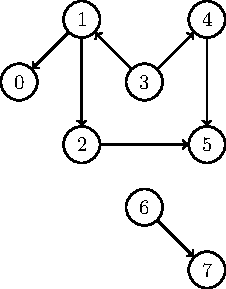
\includegraphics[scale=.8]{assets/chapter6/evaluateGraph.pdf}
    \caption{Visualisation of the graph data structure used to evaluate BST algorithms.}
    \label{evalGraph}
\end{figure}

\section{Presentable}

The last goal was that Psnodig should be presentable. We want to see if we can transpile the source programs we write to the presentation-only formats pseudocode and flowcharts.

\subsection{Pseudocode Writer}

The pseudocode writer aims to convert Psnodig ASTs to pseudocode. The writer gives us a LaTeX file by default, accompanied by the compiled result in a PDF if we wish. In this section, we will ignore the LaTeX files, and only look at the compiled versions. \\

The PDFs take up a considerable amount of space, so for readability reasons we will only present the ones relating to search algorithms. The rest will be located in \Cref{appendixB}.

\subsubsection{Search Algorithms}

\begin{figure}[ht!]
    \centering
    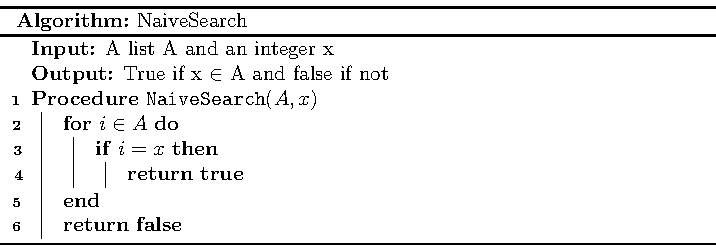
\includegraphics[scale=.8]{assets/chapter6/search/NaiveSearch_tbp.pdf}
    \caption{The result of transpiling \Cref{naiveSearchGourmet} to pseudocode.}
    \label{naiveSearchTBP}
\end{figure}

\begin{figure}[ht!]
    \centering
    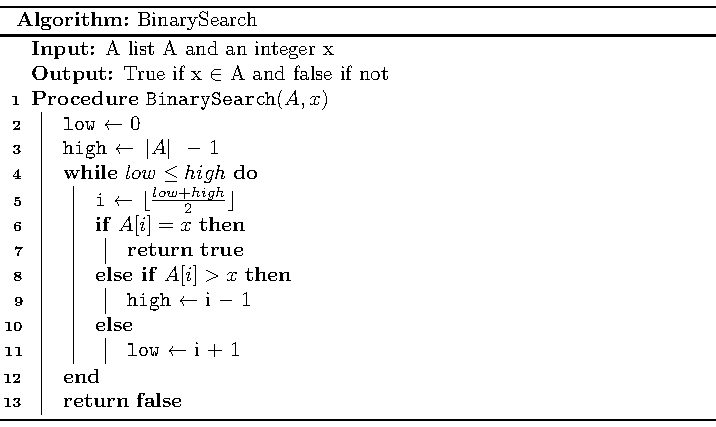
\includegraphics[scale=.8]{assets/chapter6/search/BinarySearch_tbp.pdf}
    \caption{The result of transpiling \Cref{binarySearchGourmet} to pseudocode.}
    \label{binarySearchTBP}
\end{figure}

\subsection{Flowchart Writer}

The flowchart writer is the most advanced of the four, working on yet another level of abstraction. The flowchart writer aims to convert Psnodig ASTs to flowcharts. Again, we receive a LaTeX file by default, but for the sake of evaluation we are only interested in the compiled results, ignoring the original LaTeX files. \\

As is the case with the TBP results, the IBP results span across a considerable amount of pages, and for readability reasons we will only present the ones relating to search algorithms. The rest will be located in \Cref{appendixC}.

\subsubsection{Search Algorithms}

\begin{figure}[ht!]
    \centering
    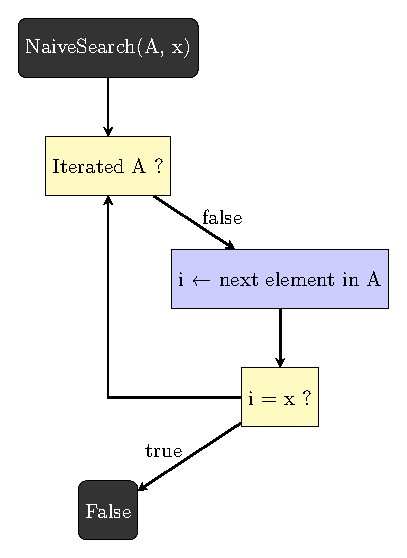
\includegraphics[scale=.7]{assets/chapter6/search/NaiveSearch_ibp.pdf}
    \caption{The result of transpiling \Cref{naiveSearchGourmet} to a flowchart.}
    \label{naiveSearchIBP}
\end{figure}

\begin{figure}[ht!]
    \centering
    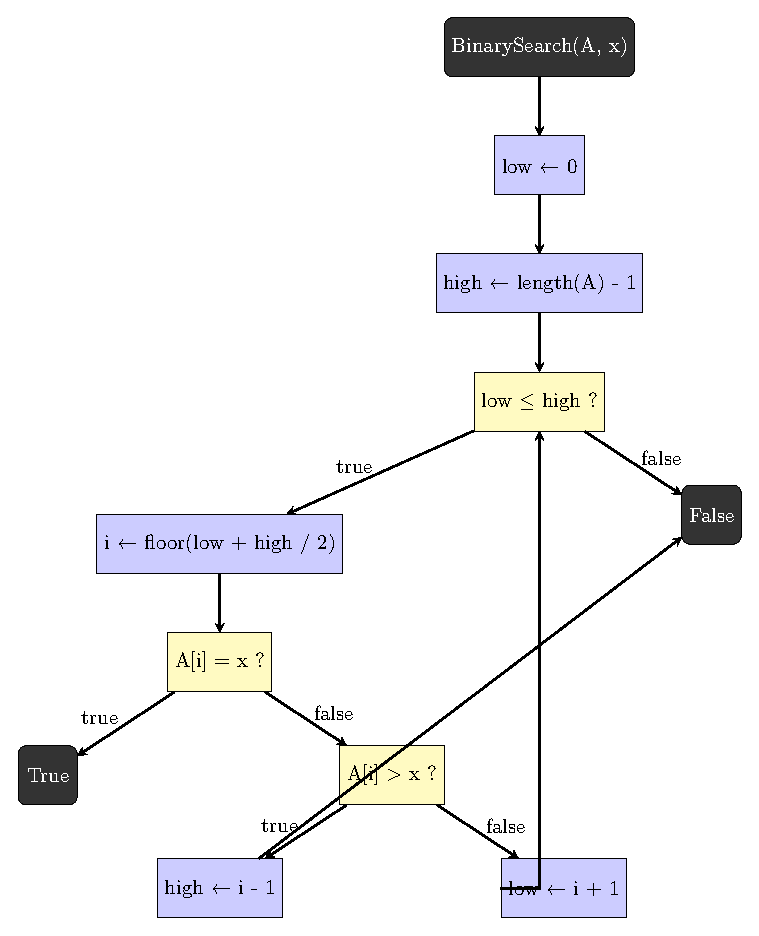
\includegraphics[scale=.65]{assets/chapter6/search/BinarySearch_ibp.pdf}
    \caption{The result of transpiling \Cref{binarySearchGourmet} to a flowchart.}
    \label{binarySearchIBP}
\end{figure}
